\chapter{Scenario Editor}

\section{Server}
Scenarios (story events) in \ourgame{} will include a number of 2D assets, 3D assets, and text. A server-side system with database integration will be implemented to make the management of data for these scenarios much easier. This will be achieved using \textbf{OpenShift}, a free platform for hosting web applications; and \textbf{Django}, an open source Python web framework that implements the model-view-controller convention.

A Django server will be used to store all scenarios and assets. A search system will be implemented for this data in order to allow for faster data retrieval. The search system will use various attributes in order to filter data. These attributes include IDs, keywords and tags.

Each member of \ourteam{} will have an account on the Django server. When a member of the team logs into the system, they will have access to the scenarios which they have created using the tool. From here, the scenarios can be opened and changed using the editor. When a scenario is being edited, it will be automatically saved each time a change to the data model of the scenario is made. The user can also manually save the scenario, which will cause the server to make a commit to a remote git repository hosted on Gitlab.com. Using a repository allows for a record to be automatically kept of all changes made to scenarios. The repository also serves as a backup of all scenario files created using the editor.

Art asset files will be uploaded through the scenario editor and committed to the repository on Gitlab. When the files are uploaded, they will be tagged with their corresponding type, such as "furniture mesh" or "item sprite". Attributes pertaining to the content type will be added as an entry in a MySQL database on the server. For example, if an item sprite were being uploaded, the properties for that item -- its name, how it can be used, what it can be used with -- would be specified in the database along with a reference to the sprite file to allow for easy searching and sorting.

\section{User Interface}
The scenario editor will feature a reactive JavaScript-based user interface. The interface will be comprised of three main elements; the navigation bar, the list view and the editor view. The navigation bar will be comprised of links to each of the major sections in the scenario editor. The list view will contain a list of data relevant to the current context. The editor view will contain information and inputs related to the item currently being edited. The major sections of the scenario editor are Conversations, Characters, Rooms, Items, and the Asset Uploader. 

Mockups for different views of the Scenario Editor can be found in Appendix \ref{app:mockups}.

\subsection{Conversations}
The conversations section will contain tools to create and edit conversations between characters. The user can add lines of dialogue associated with particular characters, and create choices for the player, which can change the outcome of the current dialogue or the entire scenario.
\subsubsection{Triggers}
When editing conversations team members will be able to add triggers into the dialog tree. Triggers correspond to functions which will be executed in the game. When a trigger is added to the conversation, the user will also specify the appropriate arguments for the function. These arguments will be later parsed in \ourgame{} and used when executing the associated function. Example uses for a trigger include attaching an emote to a character, or changing the state of a character.

\subsection{Characters}
The characters section of the scenario editor will allow the user to specify characters for the scenario. From here the user can set information about the character, such as the character's name or appearance. To define a character's appearance, the user can specify component assets, either by choosing a specific asset, or by specifying a tag. If a tag is specified, the game will choose an asset at random from all assets tagged with the specified tag when loading the scenario.
\subsubsection{States}
The user can specify states for each character. Each state has an associated conversation, and each character will start in a default state. For example, a player may talk to a character once, and in that first conversation the player will make a choice to help the character. This choice will activate a trigger that changes the state of the character. In this new state, the character now asks the player if they have completed the task yet.


\clearpage
\subsection{Rooms}
The rooms section of the scenario editor will allow the user to specify rooms required for the scenario. The system will be designed that the range of room customization can be very small or very large. This is due to to the fact that some scenarios may require very specific rooms while others may not require any specifics at all. The system will allow for the requirement that certain characters be in certain rooms. This requirement also extends to items related to the scenario. The user can also specify the type of each of the rooms. This is done through the use of tags. For example, if a room is tagged with "washroom", then when it is generated in the game, the room will only contain furniture pieces that have also been tagged with "washroom".

\subsection{Items}
Many scenarios will require the player to interact with certain items. In the items section of the editor, the user can create items to be use as part of the scenario. The item's name, description, art asset, and uses can be specified.

\subsection{Asset Uploader}
The asset uploader section will allow for the uploading of multiple asset types. The type of the content being uploaded will first be selected. Once the selection is made, the attributes pertaining to the specified asset type will be displayed. Once the file is added and the required attributes are set, the data will be sent to the server, where a descriptor file will be generated and committed to Gitlab along with the asset file itself.

\begin{figure}[H]
	\centering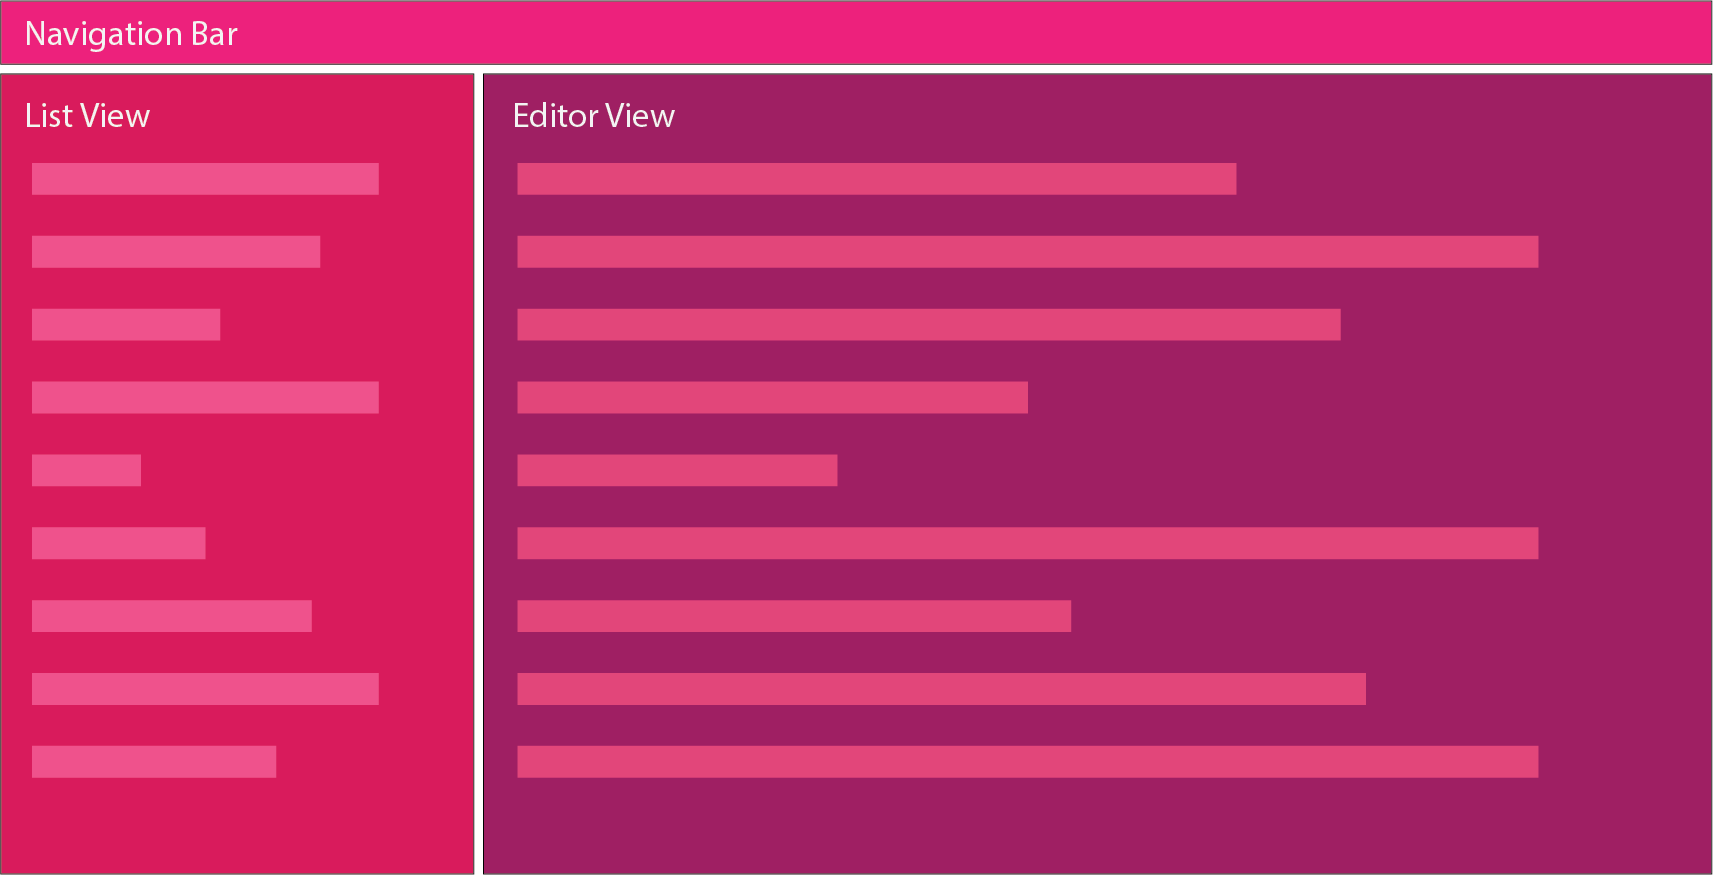
\includegraphics[width=.7\linewidth]{images/scenario_editor_sections}
	\caption{Scenario Editor Sections}
	\label{fig:scenario_sections}
\end{figure}

\subsection{AngularJS}
Creating a complex dynamic web application can become very complicated very quickly. In order to mitigate this problem AngularJS will be used. AngularJS is an open source JavaScript library which follows the Model View Whatever convention (as in "whatever works for you"). AngularJS makes the management of JavaScript data models much simpler by doing a lot of the work itself.

\subsubsection{Two Way Data Binding}
One of the major features of Angular is two way data binding. This allows for certain content to be kept in sync on both the HTML and JavaScript side. When a value is updated in the JavaScript the change will be propagated to the HTML of the application. This feature greatly reduces the amount of effort required to create a dynamic web application.

\subsubsection{JSON}
Scenarios will be stored as JSON. JSON is a simple file format which is widely supported and easily parsed. AngularJS can easily convert JavaScript data objects to JSON. This JSON can then be saved as a file and later read in \ourgame{}

\section{Data Model}
\subsection{Scenario}
The scenario object will contains collections of top level objects that can be included in scenarios, including rooms, characters, conversations, and items. It will also contain JSON that will keep track of the player's progress in a scenario, which will be combined with the  other scenarios loaded in the current play session. Refer to Appendix~\ref{app:DataModel} for a detailed diagram describing the entire data model of \ourgame{}'s scenarios. The following describes the attributes of objects involved in the data model.

\begin{description}
\item[name]{the name of the scenario}
\item[description]{a description of the scenario}
\item[rooms]{a collection of rooms included in the scenario}
\item[chracters]{a collection of characters included in the scenario}
\item[conversations]{a collection of conversations included in the scenario}
\item[items]{a collection of items included in the scenario}
\item[saveFileJson]{JSON data related to the current state of the scenario}
\end{description}

\begin{figure}[H]
\label{fig:conceptual_data_model}
\centering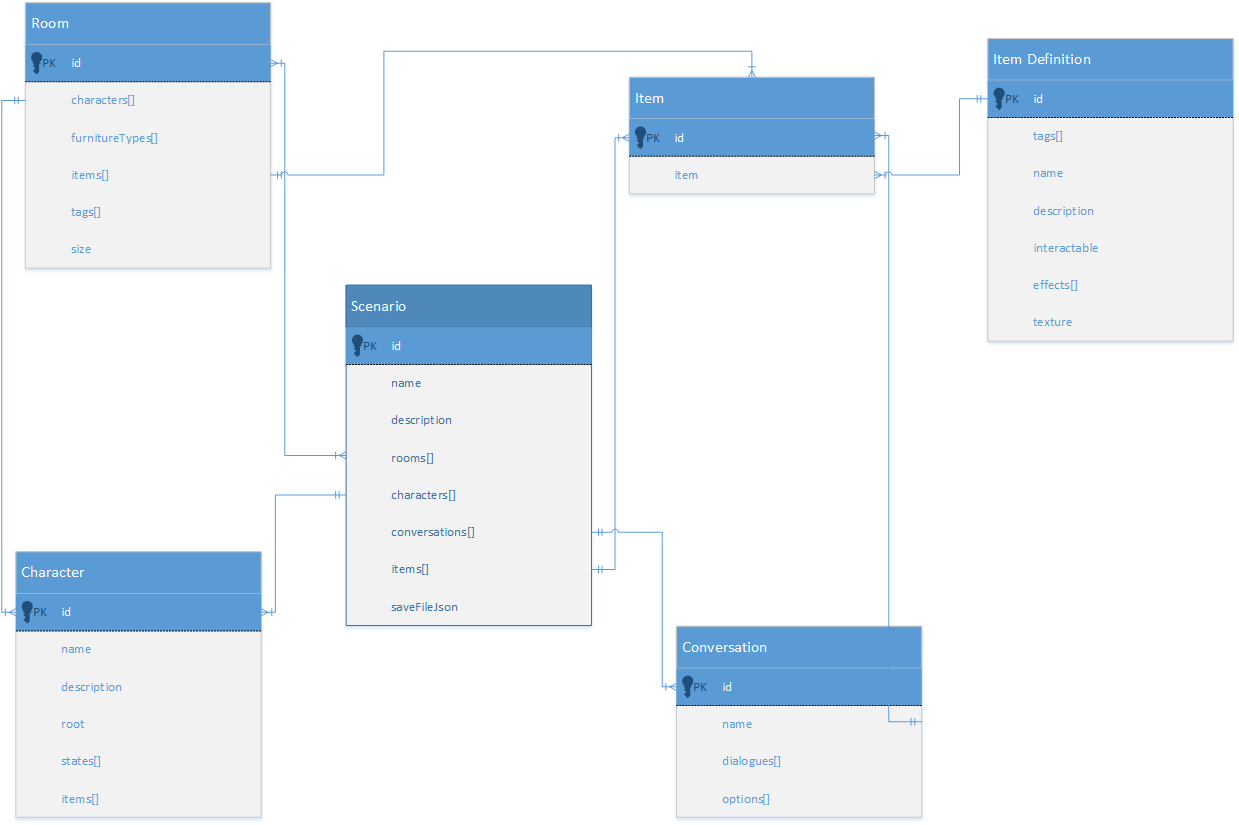
\includegraphics[width=.7\linewidth]{images/Conceptual_DataModel}
\caption{Conceptual Data Model of Scenarios}
\end{figure}

\subsection{Tag}
\begin{description}
\item[name]{the name of the tag}
\item[description]{a description of the tag}
\end{description}

\subsection{Character}
\begin{description}
\item[name]{the name of the character}
\item[description]{a description of the character}
\item[root]{the skeletal connection to the root component of the character (e.g. pelvis)}
\item[states]{a collection of states the character can be in during a scenario}
\item[items]{a collection of items a character possesses}
\end{description}

\subsubsection{Skeletal Connection}
\begin{description}
\item[component]{a character component}
\item[outComponents]{a collection of child Character Components of this object's own Character Component}
\end{description}

\subsubsection{Character Component}
\begin{description}
\item[name]{the name of the component}
\item[texture]{the URL of the image of the component}
\item[inJoint]{joint where the Character Component can be attached to}
\item[outJoints]{a collection of joints where child components can attach themselves to}
\item[tags]{a collection of tags that the component can be selected by}
\end{description}

\subsection{Conversation}
\begin{description}
\item[name]{the name of the conversation}
\item[dialogues]{a collection of dialogues spoken in the conversation by NPCs}
\item[options]{a collection of possible choices the player can choose at the end of a conversation}
\end{description}

\subsubsection{Dialogue}
\begin{description}
\item[speaker]{the character who will speak the dialogue}
\item[lines]{a collection of text to be spoken, separated by a \textbf{Next} button}
\item[triggerCalls]{a collection of calls to a trigger}
\item[conditionChecks]{a collection of conditions that can call a trigger if the condition is met}
\end{description}

\subsubsection{Trigger}
\begin{description}
\item[name]{the name of the trigger}
\item[description]{a description of the trigger}
\item[numArgs]{number of arguments the trigger is expecting}
\end{description}

\subsubsection{Trigger Call}
\begin{description}
\item[triggerId]{the id of the trigger to be called}
\item[arguments]{arguments to be sent to the trigger}
\end{description}

\subsubsection{Option}
\begin{description}
\item[text]{the option to be displayed to the player}
\item[link]{a reference to a conversation that will follow if the player chooses this option. If empty, the conversation ends and the Dialogue UI will close.}
\end{description}

\subsection{Item}
\begin{description}
\item[item]{a definition object containing properties of the item}
\end{description}

\subsubsection{Item Definition}
\begin{description}
\item[tags]{a collection of tags the item can be selected by}
\item[name]{the name of the item}
\item[description]{a description of the item}
\item[interactable]{a flag indicating whether the object can be picked up}
\item[effects]{a collection of effects the item can have on the scenario it belongs to}
\item[texture]{a URL to the image of the item}
\end{description}

\subsection{Room}
\begin{description}
\item[characters]{a collection of characters inside the room}
\item[furnitureTypes]{a collection of furniture inside the room}
\item[items]{a collection of items inside the room}
\item[tags]{a collection of tags describing the room type}
\item[size]{the dimensions of the room}
\end{description}

\subsubsection{Furniture Components}
\begin{description}
\item[name]{the name of the furniture component}
\item[meshUrl]{the path to the furniture component mesh}
\item[connections]{a collection of locations as to where the component should connect at}
\item[tags]{a collection of tags the furniture component can be selected by}
\item[types]{a collection of Furniture Types that can use the furniture component}
\end{description}

\subsubsection{Furniture Type}
\begin{description}
\item[tags]{a collection of tags describing the furniture}
\item[name]{then name of the furniture}
\end{description}

